\documentclass[8pt]{beamer}
\usefonttheme[onlymath]{serif}


\setbeamertemplate{frametitle}{%
  \vskip1ex
  \usebeamerfont{frametitle}%
  \insertsubsectionhead\par        %  ← 원하는 대로 변경 가능
  \vskip1ex
  \hrule                             % 밑줄(선택)
}

% 테마 선택 (선택 사항)
% \usetheme{Madrid} % 기본 테마, 다른 테마 사용 가능
% \font{serif}
\usepackage{amsfonts}
\usepackage{amssymb}
\usepackage[T1]{fontenc} % To use combination of textbf, textit


% \setcounter{MaxMatrixCols}{20}

% (필요한 패키지들)
% \usepackage{amsthm}
\setbeamertemplate{theorems}[numbered]  % 정리, 정의 등에 번호를 달아줌

% \theoremstyle{plain} % insert bellow all blocks you want in italic
% \newtheorem{theorem}{Theorem}[section] % to number according to section
% 
% \theoremstyle{definition} % insert bellow all blocks you want in normal text
% \newtheorem{definition}{Definition}[section] % to number according to section
% \newtheorem*{idea}{Proof idea} % no numbered block

\newtheorem{proposition}[theorem]{Proposition}

\usepackage{tcolorbox}

% 필요할 경우 패키지 추가
\usepackage{graphicx} % 이미지 삽입을 위한 패키지
\usepackage{amsmath}   % 수식 사용
\usepackage{hyperref}  % 하이퍼링크 추가
\usepackage{cleveref}
\usepackage{multicol}  % 여러 열 나누기
\usepackage{ulem} % 취소선 및줄 나누기



\newcommand{\mrm}[1]{\mathrm{#1}}
\newcommand{\mbb}[1]{\mathbb{#1}}
\newcommand{\mb}[1]{\mathbf{#1}}
\newcommand{\mc}[1]{\mathcal{#1}}
\newcommand{\tb}[1]{\textbf{#1}}
\newcommand{\ti}[1]{\textit{#1}}
\newcommand{\mypois}[1]{\operatorname{Pois}(#1)}

\newcommand{\myber}[1]{\operatorname{Bern}\!\left(#1\right)}
\newcommand{\mybin}[2]{\operatorname{Bin}\!\left(#1,#2\right)}
\newcommand{\mytoinf}[1]{#1 \rightarrow \infty}
\newcommand{\myexp}[1]{\exp{\left(#1\right)}}
\newcommand{\myunif}[2]{\operatorname{Unif}\!\left(#1, #2\right)}
\newcommand{\mygeom}[1]{\operatorname{Geom}\!\left(#1\right)}
\newcommand{\myexpo}[1]{\operatorname{Expo}\!\left(#1\right)}
\newcommand{\abs}[1]{\left\lvert #1 \right\rvert}
\newcommand{\expec}[1]{\operatorname{E}\left[ #1 \right]}
\newcommand{\myvar}[1]{\operatorname{Var}\left[#1\right]}
\newcommand{\myskew}[1]{\operatorname{Skew}\!\left[#1\right]}
\newcommand{\mykurt}[1]{\operatorname{Kurt}\!\left[#1\right]}
\newcommand{\mywei}[2]{\operatorname{Wei}\!\left(#1, #2\right)}



% 발표 제목, 저자, 날짜 설정
\title{Probability}
\author{Gwanwoo Choi}
% \date{}

\begin{document}
% 표지 슬라이드
\begin{frame}
    \titlepage
\end{frame}

% % 목차 슬라이드
% \begin{frame}
%     \frametitle{Table of Contents}
%     \tableofcontents
% \end{frame}

\subsection{Summaries of a distribution}

\begin{frame}
    \frametitle{Table of Contents}
    \tableofcontents[currentsubsection]
\end{frame}


\begin{frame}{a}
    \begin{definition}[Median]
        We say that $c$ is a \tb{median} of a random variable $X$ if $P(X\leq c) \geq 1/2$ and $P(X \geq c) \geq 1/2$. (The simplest way this can happen is if the CDF of $X$ hits $1/2$ exactly at $c$, but we know that some CDFs have jumps.)
    \end{definition}

    \begin{definition}[Mode]
        For a discrete r.v. $X$, we say that $c$ is a \tb{mode} of $X$ if it maximizes the PMF: $P(X=c) \geq P(X = x), \forall x$. For a continuous r.v. $X$ with PDF $f$, we say that $c$ is a mode if it maximizes the PDF: $f(c) \geq f(x), \forall x$.
    \end{definition}

    \begin{itemize}
        \item The median and mode of an r.v. depend only on its \ti{distribution}.
        \item A distribution can have multiple medians and multiple modes.
    \end{itemize}

    \begin{figure}
        \centering
        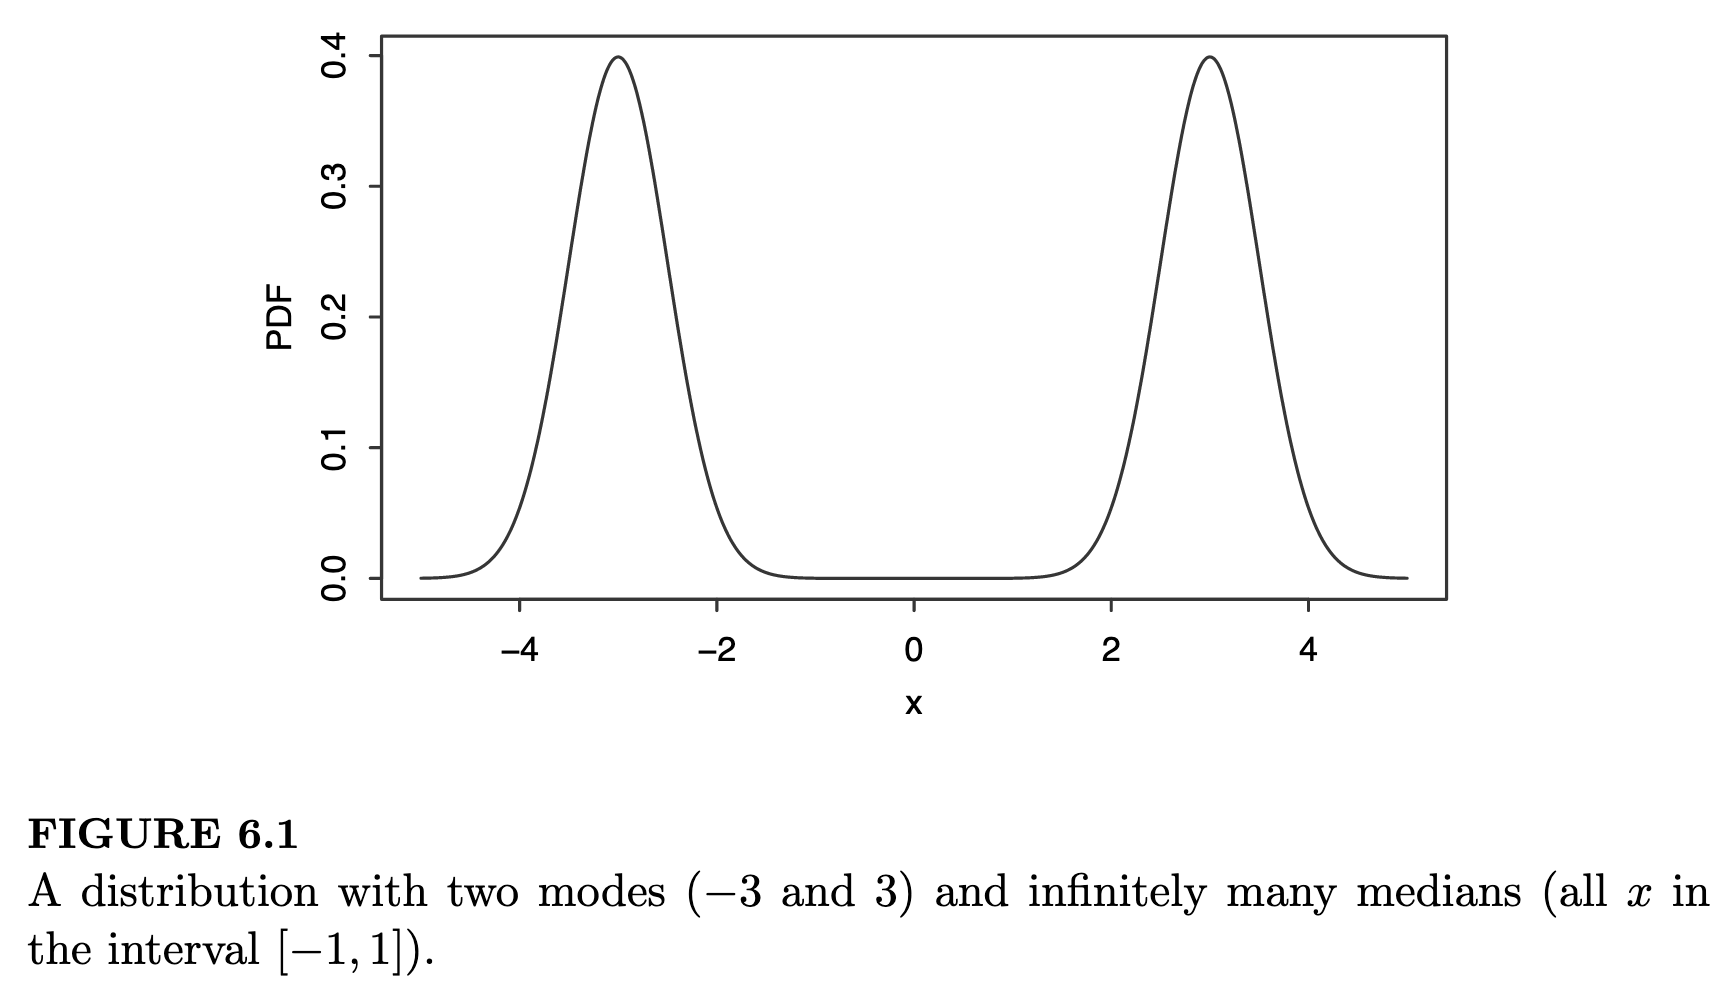
\includegraphics[width=0.55\textwidth]{fig1.png}
    \end{figure}
\end{frame}

\begin{frame}{a}
    \begin{example}[Mean, median, and mode for salaries]
        A certain company has $100$ employees. Let $s_1, s_2, \cdots, s_{100}$ be their salaries, sorted in increasing order. Let $X$ be the salary of a randomly selected employee (chosen uniformly). What is the most useful one-number summary of the salary data?
    \end{example}

    \begin{itemize}
        \item mode
        \begin{itemize}
            \item If the salaries are all different, then there exists $100$ different modes. 
            \item If there are only a few possible salaries in the company, the mode becomes more useful.
            \item But it could be also bad situation in such case. For example, 34 people receive salary $a$, 33 receive salary $b$ and 33 receive receive salary $c$.
        \end{itemize}
        \item median 
        \begin{itemize}
            \item Each number $s_{50}$ and $s_{51}$ can be median number.
            \item Any number $m$ such that $s_{50} \leq m \leq s_{51}$ can becomes median ($\because P(X \leq m) \geq 1/2, P(X \geq m) \geq 1/2$)
            \item Usual convention is to choose $m = (s_{50}+s_{51})/2$
        \end{itemize}
        \item mean
        \begin{itemize}
            \item Mean is more sensitive than the median. Consider the situation salary of CEO has slightly changed.
            \item On the other hand, suppose that we want to know the total cost the company is paying for its employees' salaries. If we only know a mode or a median, we can't extract this information.
        \end{itemize}
    \end{itemize}
\end{frame}

\begin{frame}{a}
    Suppose that we are trying to guess what a not-yet-observed r.v. $X$ will be, by making a prediction $c$. The mean and the median both seem like natural guesses for $c$, but which is better? It depends on \tb{how "better"} is defined.

    \begin{theorem}
        Let $X$ be an r.v. with mean $\mu$, and let $m$ be a median of $X$.
        \begin{itemize}
            \item The value of $c$ that minimizes the mean squared error $E[(X-c)^2]$ is $c=\mu$.
            \item The value of $c$ that minimizes the mean absolute error $E[\vert X-c \vert]$ is $c=m$.
        \end{itemize}
    \end{theorem}

    \textit{Proof.} We will first prove a useful identity $E[(X-c)^2] = Var[X] + (\mu -c)^2$. This can be drived by $Var[X] = Var[X-c] = E[(X-c)^2] - E[X-c]^2 = E[(X-c)^2] - (\mu - c)^2$. Then we can see that $E[(X-c)^2]$ is convex for $c$ and has global minimum at $c = \mu$.

    \bigskip
    \textit{Proof.} We need to show that $\forall a, \expec{\abs{X-m}} \leq \expec{\abs{X-a}}$.
    Assume $m < a$. If $X \leq m$ then $\abs{X -a} - \abs{X - m} = a - X - (m - X) = a -m$ and if $X > m$ then $\abs{X-a} - \abs{X-m} \geq m - a$. Let define r.v. $Y = \abs{X-a} - \abs{X-m}$ and indicator r.v. $I$ for $X \leq m$ (so, $1-I$ is the indicator r.v. for $X>m$). Then
    \[
    \begin{aligned}
        \expec{Y} &= \expec{YI} + \expec{Y(1-I)} \geq (a-m)\expec{I} + (m-a)\expec{(1-I)} \\
        &= (a-m)P(X\leq m) + (m-a)P(X > m) = (a-m)\{2P(X\leq m) - 1\} \\
        &\geq 0
    \end{aligned}
    \]
    And this implies $\expec{\abs{X-m}}\leq \expec{\abs{X-a}}$

\end{frame}

\subsection{Moments}

\begin{frame}
    \frametitle{tableofcontents}
    \tableofcontents[currentsubsection]
\end{frame}

\begin{frame}{a}
    \begin{definition}[Kinds of moments]
        Let $X$ be an r.v. with mean $\mu$ and variance $\sigma^2$. For any positive integer $n$, the $n$th \tb{moment} of $X$ is $E[X^n]$, the $n$th \tb{central moment} is $\expec{(X-\mu)^n}$, and the $n$th \tb{standardized moment} is $\expec{\left(\frac{X-\mu}{\sigma}\right)^n}$. Throughout the previous sentence, "if it exists" is left implicit.
    \end{definition}

    \bigskip
    The term \ti{moment} is borrowed form physics.
    \begin{figure}
        \centering
        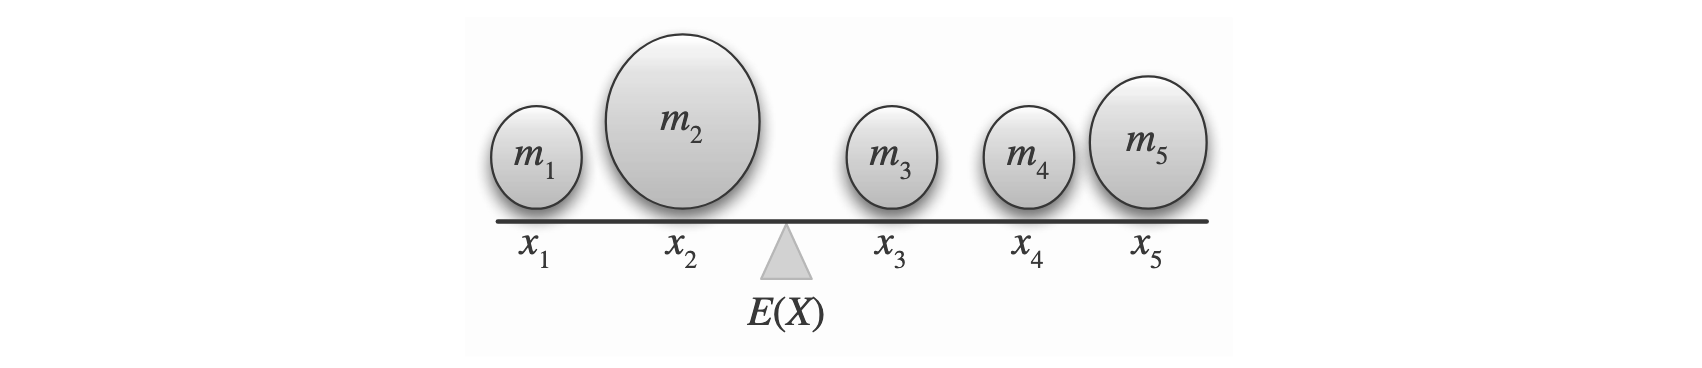
\includegraphics[width=0.5\textwidth]{fig2.png}
    \end{figure}
    Let $X$ be a discrete r.v. with distinct possible values $x_1, \dots, x_n$, and imagine a pebble with mass $m_j = P(X=x_j)$ positioned at $x_j$ on a number line, for each $j$.
    $\expec{X} = \sum_{j=1}^n m_j x_j$ is called the \ti{center of mass} of the system, and $\myvar{X} = \sum_{j=1}^n m_j (x_j - \expec{X})^2$ is called the \ti{moments of inertia} about the center of mass.

\end{frame}

\begin{frame}{a}
    \begin{definition}[Skewness]
        The \tb{Skewness} of an r.v. $X$ with mean $\mu$ and variance $\sigma^2$ is the third standardized moment of $X$.
        \[
            \myskew{X} = \expec{\left(\frac{X-\mu}{\sigma} \right)^3}
        \]
    \end{definition}
    \begin{itemize}
        \item Skewness is not depend on the location $\mu$ or the scale $\sigma$ by standardizing.
    \end{itemize}
    Why skewness measures \ti{asymmetry}?

    \begin{definition}[Symmetry of an r.v.]
        We say that an r.v. $X$ has a \ti{symmetric distribution about} $\mu$ if $X - \mu$ has the same distribution as $\mu - X$. If $X$ is symmetric about $\mu$, then
        \[
            \expec{X} - \mu = \expec{X - \mu} = \expec{\mu - X} = \mu - \expec{X} \implies \mu = \expec{X}
        \]
        Also, $\mu$ also becomes median. $P(X-\mu \leq 0) = P(\mu - X \leq 0) \implies P(X \leq \mu) = P(X \geq \mu)$
        \[
        \begin{gathered}
            P(X \leq \mu) = 1 - P(X > \mu) \geq 1 - P(X \geq \mu) = 1- P(X \leq \mu) \\
            \implies P(X \leq \mu) \geq \frac{1}{2}, P(X \geq \mu) \geq \frac{1}{2}
        \end{gathered}
        \]
        inequation is used for discrete r.v.
    \end{definition}
\end{frame}


\begin{frame}{Moments}
    \begin{lemma}[Symmetry in terms of the PDF]
        Let $X$ be a continuous r.v. with PDF $f$. Then $X$ is symmetric about $\mu$ if and only if $f(x) = f(2\mu - x)$ for all $x$.
    \end{lemma}

    \ti{Proof.}
    \begin{itemize}
        \item $X$ is symmetric about $\mu \implies f(x) = f(2\mu - x)$. 
        \[
        \begin{gathered}
            F(x) = P(X- \mu \leq x - \mu)  = P(\mu - X \leq x - \mu) \\
            = P(X > 2\mu - x) = 1 - F(2\mu - x)
            \implies f(x) = f(2\mu - x)
        \end{gathered}
        \]
        \item $f(x) = f(2\mu - x) \implies X$ is symmetric about $\mu$
        \[
        \begin{gathered}
            P(X-\mu \leq t) = \int_{-\infty}^{\mu +t} f(x) dx = \int_{-\infty}^{\mu +t} f(2\mu - x)dx = \int_{\mu - t}^{\infty} f(x) dx \\
            = P(X \geq \mu - t) = P(\mu -X \leq t)
        \end{gathered}
        \]
    \end{itemize}
\end{frame}

\begin{frame}{Moments}
    \begin{lemma}[Odd central moments of a symmetric distribution]
        Let $X$ be symmetric about its mean $\mu$. Then for any odd number $m$, the $m$th central moment $\expec{(X-\mu)^m}$ is $0$ if it exists.
    \end{lemma}

    \ti{Proof.}
    Since $X-\mu$ has the same distribution as $\mu -X$, they have the same $m$th moment (if it exists):
    \[
    \begin{gathered}
        \expec{(X-\mu)^m} = \expec{(\mu - X)^m} = \expec{(-1)^m (X -\mu)^m} = - \expec{(X - \mu)^m} \\
        \implies \expec{(X - \mu)^m} = 0
    \end{gathered}
    \]

    \begin{itemize}
        \item THis leads us to consider using an odd standardized moment as a measure of skew of a distribution.
        \item If $m = 1$, $\expec{\frac{X - \mu}{\sigma}} = \frac{1}{\sigma} (\expec{X} - \mu) = 0$
        \item So we use \tb{third standardized moment} $\expec{\left(\frac{X - \mu}{\sigma}\right)^3}$ as measurement of skewness
        \item Positive skewness $\expec{\left(\frac{X - \mu}{\sigma}\right)^3} > 0$ indicates that distribution has a long right tail relative to the left tail. Negative skewness indicates reverse.
        \item The \tb{inverse of above is false}, since there exist asymmetric distributions whose odd central moments are all $0$
    \end{itemize}
\end{frame}

\begin{frame}{Moments}
    \begin{itemize}
        \item Another important descriptive feature of a distribution is how heavy its tails are.
        \item As with measuring skew, no single measure can perfectly capture the tail behavior, but there is a widely used summary based on the fourth standardized moment.
    \end{itemize}
    \begin{definition}[Kurtosis]
        The \tb{kurtosis} of an r.v. $X$ with mean $\mu$ and variance $\sigma^2$ is a shifted version of the fourth standardized moment of $X$
        \[
        \mykurt{X} = \expec{\left(\frac{X-\mu}{\sigma}\right)^4} - 3
        \]
    \end{definition}
    \begin{itemize}
        \item The reason for subtracting $3$ is that this makes any Normal distribution have kurtosis $0$
        \item However, some source define the kurtosis without the $3$, in which case they call our version "excess kurtosis"    
    \end{itemize}
\end{frame}

\begin{frame}{Moments}
    \begin{figure}
        \centering
        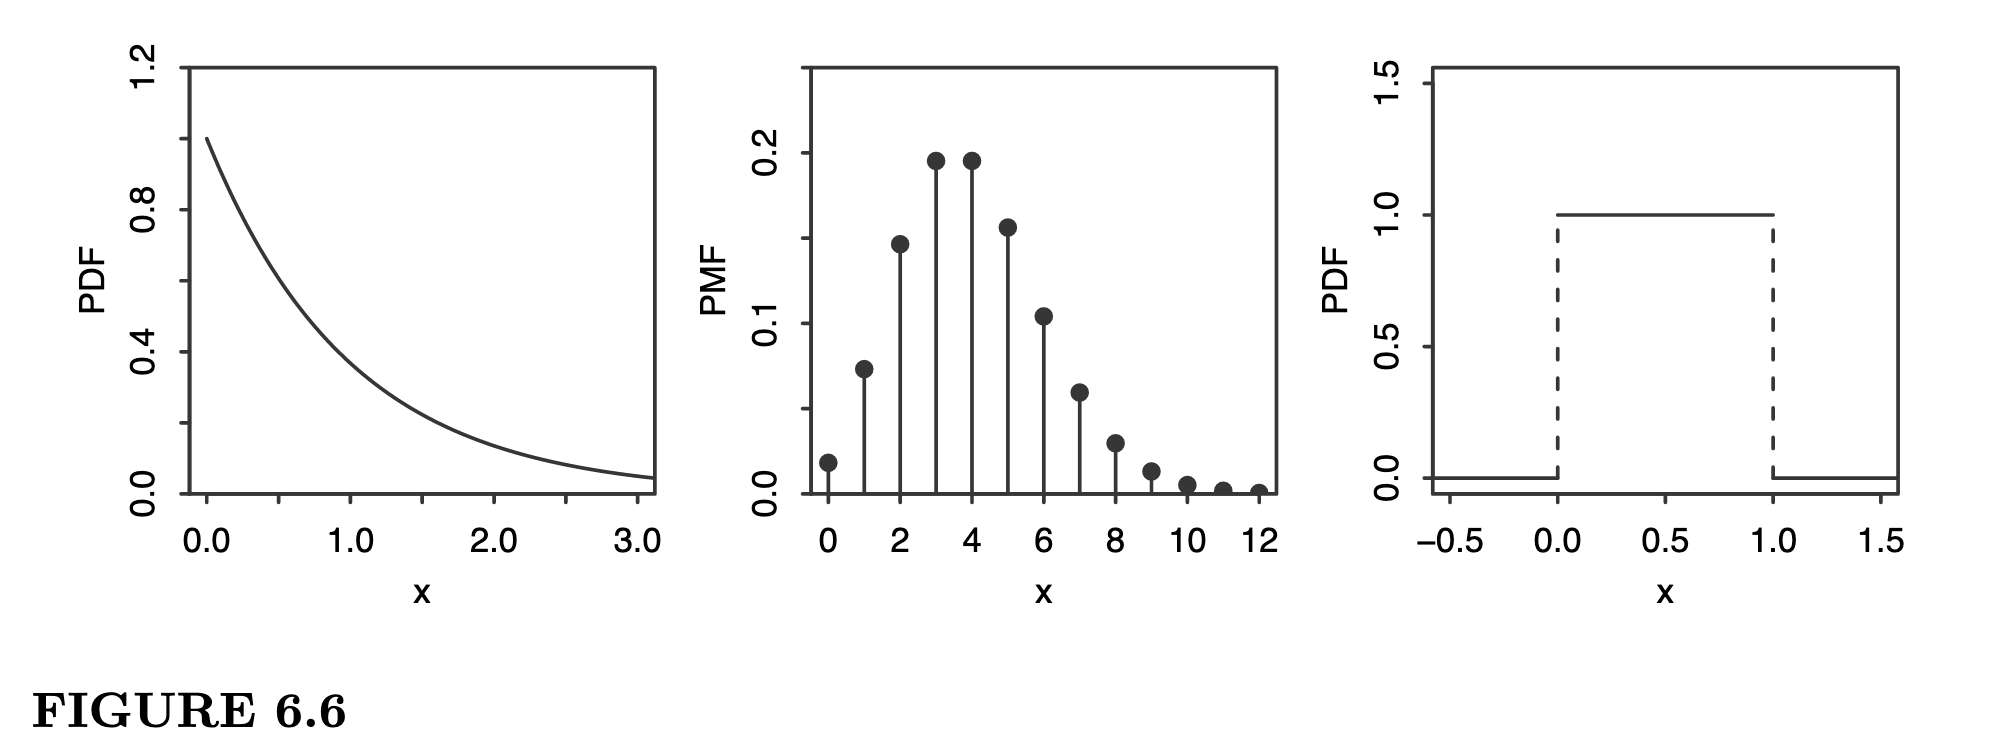
\includegraphics[width=0.8\textwidth]{SkewAndKurtosis.png}
    \end{figure}

    Skewness and kurtosis of named distribution, $\myexpo{1}, \mypois{4},$ and $\myunif{0}{1}$
    \begin{itemize}
        \item $\myexpo{1}$: skewness = $2$, kurtosis = $6$
        \item $\mypois{4}$: skewness = $0.5$, kurtosis = $0.25$
        \item $\myunif{0}{1}$: skewness = $0$, kurtosis = $-1.2$
    \end{itemize}
\end{frame}

\subsection{Sample Moments}
\begin{frame}{Sample moments}
    \begin{itemize}
        \item How to estimate unknown parameters of distribution?
        \item It is especially common to want to estimate the mean and variance of a distribution
    \end{itemize}

    \begin{definition}[Sample Moments]
        Let $X_1, \dots, X_n$ be i.i.d. random variables.
        The $k$th \tb{sample moment} is the r.v.
        \[
        M_k = \frac{1}{n} \sum_{j=1}^n X_j^k
        \]
    \end{definition}

    The \tb{sample mean} $\bar{X_n}$ is the first sample moment
    \[
    \bar{X}_n = \frac{1}{n} \sum_{j=1}^n X_j
    \]

    \begin{itemize}
        \item The law of large numbers says that the $k$th sample moment of i.i.d. random variables $X_1, X_2, \dots, X_n$ converges to the $k$th moment $\expec{X_1^k}$ as $n \rightarrow \infty$.

    \end{itemize}
    \[
        \expec{\left(\frac{1}{n} \sum_{j=1}^n X_j^k\right)} = \frac{1}{n} \left(\expec{X_1^k} + \cdots + \expec{X^k_n} \right) = \frac{n}{n} \expec{X^k_1} = \expec{X^k_1}
   \]
\end{frame}

\begin{frame}{Sample Moments}
    \begin{theorem}[Mean and variance of sample mean]
        Let $X_1, \dots, X_n$ be i.i.d. r.v.s with mean $\mu$ and variance $\sigma^2$. Then the sample mean $\bar{X}_n$ is unbiased for estimating $\mu$. That is
        \[
        \expec{\bar{X}_n} = \mu
        \]
        The variance of $\bar{X}_n$ is given by
        \[
        \myvar{\bar{X}_n} = \frac{\sigma^2}{n}
        \]
    \end{theorem}

    \ti{Proof.} Expectation of $k$th sample monent is unbiased for estimating the $k$th moment.

    So $E[\bar{X}_n] = \mu$ holds.

    For the variance, the fact that the variance of the sum of \ti{independent} r.v.s is the sum of the variances
    \[
    \myvar{\bar{X}_n} = \frac{1}{n^2} \myvar{X_1 + \cdots + X_n} = \frac{n}{n^2} \myvar{X_1} = \frac{\sigma^2}{n} \qquad \blacksquare
    \]

    Note that 
    \[
    \myvar{\bar{X}_n} = \expec{(\bar{X}_n - \expec{\bar{X}_n})^2} = \expec{(\bar{X}_n - \mu)^2}
    \]
\end{frame}

\begin{frame}{Sample Moments}
    \begin{definition}[Sample variance and sample standard deviation]
        Let $X_1, \dots, X_n$ be i.i.d. random variables. The \tb{sample variance} is the r.v.

        \[
        S^2_n = \frac{1}{n-1} \sum_{j=1}^n (X_j - \bar{X}_n)^2
        \]
        The \tb{sample standard deviation} is $\sqrt{S^2_n}$
    \end{definition}

    \begin{theorem}[Unbiasedness of sample variance]
        Let $X_1, \dots, X_n$ be i.i.d. r.v.s with mean $\mu$ and variance $\sigma^2$. Then the sample variance $S^2_n$ is \tb{unbiased} for estimating $\sigma^2$, i.e.
        \[
            \expec{S^2_n} = \sigma^2
        \]
    \end{theorem}
    \begin{itemize}
        \item Note that sample standard deviation is \tb{not unbiased}, $E[\sqrt{S^2_n}] \neq \sigma$
    \end{itemize}
\end{frame}
\begin{frame}{Sample Moments}
    \begin{theorem}[Unbiasedness of sample variance]
        Let $X_1, \dots, X_n$ be i.i.d. r.v.s with mean $\mu$ and variance $\sigma^2$. Then the sample variance $S^2_n$ is \tb{unbiased} for estimating $\sigma^2$, i.e.
        \[
            \expec{S^2_n} = \sigma^2
        \]
    \end{theorem}

    Before start proof, following equation is hold
    \[
        \begin{aligned}
            \sum_{j=1}^n (X_j - c)^2 &=  \sum_{j=1}^n ((X_j - \bar{X}_n) + (\bar{X}_n - c))^2 \\
            &= \sum_{j=1}^n (X_j - \bar{X}_n)^2 + 2(\bar{X} - c) \sum_{j=1}^n (X_j - \bar{X}_n) + \sum_{j=1}^n (\bar{X}_n - c)^2 \\
            &= \sum_{j=1}^n (X_j - \bar{X}_n)^2 + \sum_{j=1}^n (\bar{X}_n - c)^2 \left(\because \sum_{j=1}^n (X_j - \bar{X}_n) = 0\right) \\
            &= \sum_{j=1}^n (X_j - \bar{X}_n)^2 + n (\bar{X}_n - c)^2
            \end{aligned}
    \]
\end{frame}

\begin{frame}{Sample Moments}
    \begin{theorem}[Unbiasedness of sample variance]
        Let $X_1, \dots, X_n$ be i.i.d. r.v.s with mean $\mu$ and variance $\sigma^2$. Then the sample variance $S^2_n$ is \tb{unbiased} for estimating $\sigma^2$, i.e.
            
        \[ \expec{S^2_n} = \sigma^2 \]
    \end{theorem}

    \ti{Proof.}
    \[
        \expec{(X_1 - \mu)^2 + \dots + (X_n - \mu)^2} = n \expec{(X_1 - \mu)^2} = n \sigma^2
    \]

    Also, 
    \[
    \begin{aligned}
        &\expec{(X_1 - \mu)^2 + \dots (X_n - \mu)^2} = \expec{\sum_{j=1}^n(X_j - \bar{X}_n)^2 + n (\bar{X}_n - \mu)^2 } \\ 
        &= \expec{\sum_{j=1}^n (X_j - \bar{X}_n)^2} + n \myvar{\bar{X}_n} = \expec{\sum_{j=1}^n (X_j - \bar{X}_n)^2} + \sigma^2 \\
        &\implies \expec{\sum_{j=1}^n (X_j - \bar{X}_n)} = (n-1) \sigma^2 \implies \expec{\frac{1}{n-1} \sum_{j=1}^n (X_j - \bar{X}_n)^2} = \sigma^2
    \end{aligned}
    \]
\end{frame}

\subsection{Moment generating function}

\begin{frame}{Moment generating functions}
    \begin{itemize}
        \item Generating functions are a powerful tool in combinatories and probability, bridging between sequences of numbers and the world of calculus
        \item Starting with a sequence of numbers, create a continuous function (the generating function) that encodes the sequence
    \end{itemize}

    A moment generating function, as its name suggests, is a generating function that encodes the \tb{moments} of a distribution.

    \begin{definition}[Moment generating function]
        The \tb{moment generating function}(MGF) of an r.v. $X$ is $M(t) = \expec{e^{tX}}$, as a functino of t, if this is finite on some open interval $(-a, a)$ containing $0$. Otherwise the MGF of $X$ does not exist.
    \end{definition}

    \begin{example}[Bernoulli MGF]
        For $X \sim \myber{p}, e^{tX}$ takes $e^t$ with probability $p$ and takes $1$ with probability $1-p$.
        \[
        M(t) = \expec{e^{tX}} = pe^t + q
        \]

        $M(t)$ is finite for interval $(-\infty, \infty)$. $M(t)$ is defined on the entirel real line.
    \end{example}
\end{frame}

\begin{frame}{a}
    \begin{example}[Geometric MGF]
        For $X \sim \mygeom{p}$,
        \[
        M(t) = \expec{e^{tX}} = \sum_{k=0}^\infty e^{tk} q^k p = p \sum_{k=0}^\infty (qe^t)^k = \frac{p}{1 - qe^t}
        \]

        $M(t)$ is finite in interval $(-\infty, \log{(1/q)})$.
    \end{example}

    \begin{example}[Uniform MGF]
        Let $U \sim \myunif{a}{b}$.
        \[
        M(t) = \expec{e^{tU}} = \frac{1}{b-a} \int_a^b e^{tu} du = \frac{e^{tb} - e^{ta}}{t (b-a)}, \forall t \neq  0, M(0) = 1
        \]
    \end{example}
\end{frame}

\begin{frame}{Moment generationg function}
    Then why is MGF important?
    \begin{itemize}
        \item The MGF encodes the moments of an r.v.
        \item The MGF of an r.v. determines its distribution (like CDF and PMF/PDF)
        \item MGFs make it easy to find the distribution of a sum of independent r.v.s.
    \end{itemize}
    \begin{theorem}[Moments via derivatives of the MGF]
        Given the MGF of $X$, we can get $n$th moment of $X$ by evaluating the $n$th derivative of the MGF at $0$
        \[
            \expec{X^n} = M^{(n)}(0)
        \]
    \end{theorem}

    \ti{Proof.} $M(t) = \expec{e^{tX}} = \expec{\sum_{n=0}^\infty \frac{(tX)^n}{n!}} = \sum_{n=0}^\infty \expec{X^n \frac{t^n}{n!}} = \sum_{n=0}^\infty \frac{t^n}{n!} \expec{X^n}$.
    On the other hand, by taylor series, $M(t) = \sum_{n=0}^\infty M^{(n)}(0) \frac{t^n}{n!}$. This implies $\expec{X^n} = M^{(n)}(0)$

    \begin{theorem}[MGF determines the distribution]
        If two r.v.s have the \tb{same MGF}, they must have the \tb{same distribution}. In fact, if there is even a tiny interval $(-a, a)$ containing $0$ on which the MGFs are equal, then the r.v.s must have the same distribution
    \end{theorem}
\end{frame}

\begin{frame}{MGF of a sum of independent r.v.s}
    \begin{theorem}
        If $X$ and $Y$ are independent, then the MGF of $X + Y$ is the product of the individual MGFs
        \[
        M_{X+Y} (t) = M_X (t) M_Y (t)
        \]
    \end{theorem}
    \ti{proof.} If $X$ and $Y$ are independent, then $\expec{e^{t (X+Y)}} = \expec{e^{tX}} \expec{e^{tY}}$. (this follows from results discussed in Chapter 7)

    \begin{example}[Binomial MGF]
        The MGF of a $\myber{p}$ r.v. is $pe^t +q$, so the MGF of a $\mybin{n}{p}$ r.v. is $M(t) = (pe^t + q)^n$
    \end{example}

    \begin{proposition}[MGF of location-scale transformation]
        If $X$ has MFG $M(t)$, then the MGF of $a + bX$ is 
        \[
            \expec{e^{t(a+bX)}} = e^{ta}\expec{e^{tbX}} = e^{ta}M(bt)
        \]
    \end{proposition}
\end{frame}

\begin{frame}{MGF of a sum of independent r.v.s}
    \begin{example}[Normal MGF]
        The MGF of a standard Normal r.v. $Z$ is 
        \[
        M_Z(t) = \expec{e^{tZ}} = \int_{-\infty}^\infty e^{tz} \frac{1}{\sqrt{2\pi}} e^{-z^2/2} dz = e^{t^2 /2} \int_{-\infty}^\infty \frac{1}{\sqrt{2\pi}} e^{-(z - t)^2 / 2}dz = e^{t^2/ 2}
        \]
        $X = \sigma Z + \mu$. Then MGF of $X$, $M_X$ is 
        \[
        M_X(t) = e^{\mu t} M_Z(\sigma t) = e^{\mu t} e^{(\sigma t)^2/2} = e^{\mu t + \frac{1}{2} \sigma^2 t^2} 
        \]
    \end{example}

    \begin{example}{Exponential MGF}
        The MGF of $X \sim \myexpo{1}$ is
        \[
            M_X(t) = \expec{e^{tX}} = \int_{0}^\infty e^{tx} e^{-x} dx = \int_{0}^\infty e^{-x(1 -t)} dx = \frac{1}{1 - t}, \forall t < 1
        \]
        So the MGF of $Y = X /\lambda \sim \myexpo{\lambda}$ is
        \[
        M_Y (t) = M_X(t / \lambda) = \frac{\lambda}{\lambda - t}, \forall t <\lambda
        \]
    \end{example}
\end{frame}

\subsection{Generating moments with MGFs}

\begin{frame}
    \frametitle{Table of Contents}
    \tableofcontents[currentsubsection]
\end{frame}

\begin{frame}{Generating moments with MGFs}
    \begin{example}[Exponential moments]
        Let $X \sim \myexpo{1}$. The MGF of $X$ is $M(t) = \frac{1}{1 - t} \forall t<1$. Then
        \[
        \begin{aligned}
            M(t) &= \frac{1}{1 - t} = \sum_{n=0}^\infty t^n = \sum_{n=0}^\infty n! \frac{t^n}{n!} = \sum_{n=0}^\infty M^{(n)}(0) \frac{t^n}{n!} = \sum_{n=0}^\infty \expec{X^n} \frac{t^n}{n!} \\
            &\implies \expec{X^n} = n!
        \end{aligned}
        \]
        For $Y = X / \lambda \sim \myexpo{\lambda}$, $Y^n = X^n / \lambda^n$ and $\expec{Y^n} = \frac{n!}{\lambda^n}$
    \end{example}

    \begin{example}[Standard Normal moments]
        Let $Z \sim \mathcal{N}(0, 1)$.
        \[
        \begin{aligned}
            M(t) &= e^{t^2 /2} = \sum_{n=0}^\infty \frac{(t^2/2)^n}{n!} = \sum_{n=0}^\infty \frac{t^{2n}}{2^n n!} = \sum_{n=0}^\infty \frac{(2n)!}{2^n n!} \frac{t^{2n}}{(2n)!} \\
            &\implies E[Z^{2n}] = \frac{(2n)!}{2^n n!} = \prod_{k=1}^n (2k - 1)
        \end{aligned}
        \]
        And $E[Z^{2n-1}] = 0, \forall n$. 
    \end{example}
\end{frame}

\begin{frame}{Generating moments with MGFs}
    \begin{example}[Log-Normal moments]
        We say that if $Y = e^X$ where $X \sim \mathcal{N}(\mu, \sigma^2)$, then $Y$ is \tb{Log-Normal} with parameters $\mu$ and $\sigma^2$, denoted by $Y \sim \mathcal{LN} (\mu, \sigma^2)$.

        The name \ti{Log-Normal} is originated from \tb{"Log is Normal"}, $\log{Y} = X$.
        
        Interestingly, Log-Normal MGF does not exist, since $\expec{e^{tY}}$ is infinite for all $t> 0$.

        Consider the case $Y = e^Z, Z \sim \mathcal{N}(0, 1)$. Then
        \[
            \expec{e^{tY}} = \expec{e^{te^Z}} = \int_{-\infty}^{\infty} e^{te^z} \frac{1}{\sqrt{2\pi}} e^{-z^2 /2}  = \int_{-\infty}^{\infty} \frac{1}{\sqrt{2\pi}} e^{te^z - z^2/2} dz
        \]

        $\forall t > 0, e^{te^z - z^2 /2} \rightarrow \infty $ as $z \rightarrow \infty$. $\therefore \expec{e^{tY}} = \infty$.
        
        Since $\expec{e^{tY}}$ is not finite on an open interval around $0$, the MGF of $Y$ does not exist.

        However, even though the Log-Normal MGF does not exist, we can get moments of Log-Normal, using the MGF of the Normal.
        For $Y=e^X, X \sim \mathcal{N}(\mu, \sigma^2)$,
        \[
        E[Y^n] = E[e^nX] = e^{n\mu + \frac{1}{2}n^2 \sigma^2} 
        \]
    \end{example}
\end{frame}

\begin{frame}{Generating moments with MGFs}
    Weibull distribution is widely used distributions in \ti{survival analysis} (e.g. modeling how long someone with a particular disease will live)
    \begin{example}[Weibull distribution]
        Let $T \sim X^{1/ \gamma}, X \sim \myexpo{\lambda}, \lambda,\gamma > 0$. Then the distribution of $T$ is called the \tb{Weibull distribution}, and denoted by $T \sim \mywei{\lambda}{\gamma}$.

        The PDF of $T$ is (Shown from Chapter 8)
        \[
        f(t) = \gamma \lambda e^{-\lambda t^{\gamma}}t^{\gamma -1}, \forall t > 0
        \] 

        For $\lambda = 1$ and $\gamma = 1/3$,
        \begin{itemize}
            \item Find $P(T > s+t | T> s), \forall s,t > 0$. Does $T$ have the memoryless property?
            \item Find the mean and variance of $T$, and the $n$th moment $\expec{T^n}, \forall n=1,2,\dots$
            \item Determine whether or not the MGF of $T$ exists.
        \end{itemize}
    \end{example}

    \begin{itemize}
        \item Find $P(T > s+t | T> s), \forall s,t > 0$. Does $T$ have the memoryless property?
    \end{itemize}
    \[
    \begin{gathered}
        P(T\leq t) = P(X^3 \leq t) = F_X(t^{1/3}) = 1 - e^{-t^{1/3}}, \forall t>0 \\
        \implies P(T> s+t | T>s) = \frac{1 - P(T \leq s+t)}{1 - P(t \leq s)} = \frac{e^{-(s+t)^{1/3}}}{e^{-s^{1/3}}} \neq e^{-t^{1/3}} = P(T > t)
    \end{gathered}
    \]
    $\therefore$ $T$ does not have memoryless property
\end{frame}

\end{document}